%%%%%%%%%%%%%%%%%%%%%%%%%%%%%%%%%%%%%%%
% Original author:
% Rahul Chauhan (http://rahulchauhan.net)
%
% Original repository:
% https://github.com/rahulworld/rahulworld-Resume
%%%%%%%%%%%%%%%%%%%%%%%%%%%%%%%%%%%%%%

\documentclass[]{rahulworld-resume}
\usepackage{tikz}

\begin{document}
% %%%%%%%%%%%%%%%%%%%%%%%%%%%%%%%%%%%%% With Image
% \begin{minipage}[t]{0.15\textwidth} 
% \vfill
% \begin{tikzpicture}
% 	\clip (0,0) circle (1.5cm) node {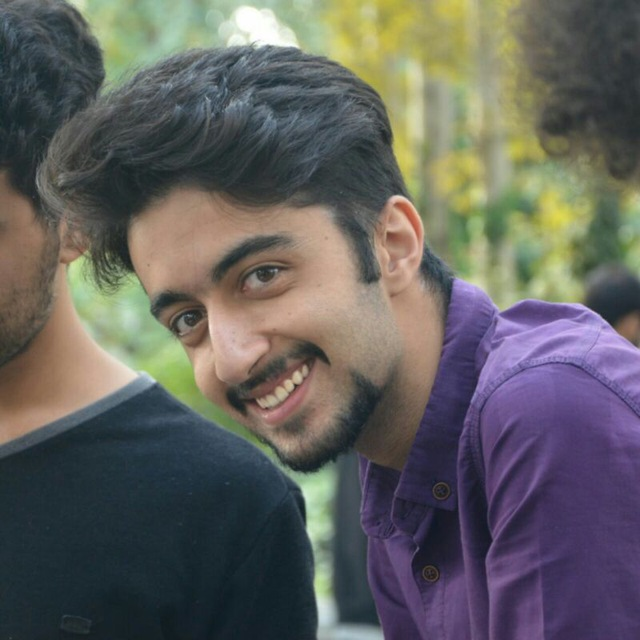
\includegraphics[width=3cm]{me.jpg}};
% \end{tikzpicture}
% \end{minipage} 
% \hfill
% \begin{minipage}[t]{0.40\textwidth} 
% \begin{large}
% 	\headername{Behzad Shayegh Boroujeni}\\
% \end{large}
% \vspace{5pt}
% University of Tehran, Tehran, Iran
% \end{minipage} 
% %%%%%%%%%%%%%%%%%%%%%%%%%%%%%%%%%%%%% Without Image
\begin{minipage}[t]{0.50\textwidth} 
	\begin{large}
		\headername{Behzad Shayegh Boroujeni}\\
	\end{large}
	\vspace{5pt}
	University of Tehran, Tehran, Iran
\end{minipage} 
%%%%%%%%%%%%%%%%%%%%%%%%%%%%%%%%%%%%%%
%%%%%%%%%%%%%%%%%%%%%%%%%%%%%%%%%%%%%% Contact
\hfill
\begin{minipage}[t]{0.35\textwidth} 
\vspace{10pt}
			\hfill \href{tel:+989381377391}{+98 938 137 73 91 \;\; 
\includegraphics[width=8pt]{icons/phone.png}}\\
\vspace{2pt}\hfill \href{mailto:behzad.shayegh.b@gmail.com}{behzad.shayegh.b@gmail.com \;\; 
\includegraphics[width=8pt]{icons/mail.png}}\\
\vspace{2pt}\hfill \href{https://github.com/BehzadShayegh}{BehzadShayegh \;\; 
\includegraphics[width=8pt]{icons/github.png}}\\
\vspace{2pt}\hfill \href{https://www.linkedin.com/in/behzad-shayegh}{behzad-shayegh \;\; 
\includegraphics[width=8pt]{icons/linkedin.png}}\\
\vspace{2pt}\hfill \href{https://behzadshayegh.github.io}{BehzadShayegh.github.io \;\; 
\includegraphics[width=8pt]{icons/website.png}}
\end{minipage} 
\vspace{20pt}
%%%%%%%%%%%%%%%%%%%%%%%%%%%%%%%%%%%%%%

%%%%%%%%%%%%%%%%%%%%%%%%%%%%%%%%%%%%%%
%
%     COLUMN ONE
%
%%%%%%%%%%%%%%%%%%%%%%%%%%%%%%%%%%%%%%

\begin{minipage}[t]{0.36\textwidth} 
	%%%%%%%%%%%%%%%%%%%%%%%%%%%%%%%%%%%%%%
	%     EDUCATION
	%%%%%%%%%%%%%%%%%%%%%%%%%%%%%%%%%%%%%%
	\section{Education}
	\vspace{-5pt}\noindent\rule{\textwidth}{0.4pt}\vspace{5pt}\\
	\hspace{-0.4cm}
	\begin{minipage}{\linewidth}
		\dirtree{%
			.1  \begin{minipage}[t]{6.83cm}\vspace{-7pt}
					\runsubsection{\large Bachelor of Science} \hfill \datecolor{2017-2022}\\
					\descript{\href{https://ut.ac.ir/en}{University of Tehran  
\includegraphics[width=8pt]{icons/redirect.png}}}
					\vspace{5pt}
				\end{minipage}.
			.2  \begin{minipage}[t]{6.27cm}\vspace{-7pt}
					\runsubsection{\normalsize Major in Computer Engineering}\\
					\small $\bullet$ Focused in Software Engineering\\
					\small $\bullet$ Thesis: Persian Address to Postal‐Code Converter (Grade: 19.88/20)\\
					\small $\bullet$ \href{https://behzadshayegh.github.io/CV/BCsCEreport.pdf}{GPA: 18.41/20 (3.93/4) 
\includegraphics[width=8pt]{icons/redirect.png}}\\
					\small $\bullet$ GPA over the last year: 18.71/20\\
					\descript{\href{https://ece.ut.ac.ir/en/ece}{{School of ECE}  
\includegraphics[width=8pt]{icons/redirect.png}}}
				\end{minipage}.
			.2  \begin{minipage}[t]{6.27cm}\vspace{-7pt}
					\runsubsection{\normalsize Minor in Computer Science}\\
					\small $\bullet$ \href{https://behzadshayegh.github.io/CV/BCsCSreport.pdf}{GPA: 19.73/20 (4/4) 
\includegraphics[width=8pt]{icons/redirect.png}}\\
					\descript{\href{https://science.ut.ac.ir/en/web/math/home}{{School of MSCS}  
\includegraphics[width=8pt]{icons/redirect.png}}}
				\end{minipage}.
		}
	\end{minipage}
	\sectionsep

	%%%%%%%%%%%%%%%%%%%%%%%%%%%%%%%%%%%%%%
	%     COURSEWORK
	%%%%%%%%%%%%%%%%%%%%%%%%%%%%%%%%%%%%%%
	\section{Relevant Courses}\vspace{-4pt}{\normalsize\normalfont * indicates graduate courses.}\vspace{-8pt}\\
	\noindent\rule{0.75\textwidth}{0.4pt}\hfill Grade/20

	Computational Neuroscience * \hfill 19.75\\
	\descriptright{\href{https://scholar.google.com/citations?user=tK6cb1AAAAAJ&hl=en}{Assoc. Prof. Mohammad Ganjtabesh 
\includegraphics[width=8pt]{icons/redirect.png}}}
	\vspace{5pt}
	Natural Language Processing * \hfill 19.1\\
	\descriptright{\href{https://ece.ut.ac.ir/en/~hfaili}{Assoc. Prof. Heshaam Faili 
\includegraphics[width=8pt]{icons/redirect.png}}}
	\vspace{5pt}
	Reinforcement Learning * \hfill 20\\
	\descriptright{\href{https://ece.ut.ac.ir/en/~mnili}{Prof. Majid Nili 
\includegraphics[width=8pt]{icons/redirect.png}}}
	\vspace{5pt}
	Statistical Machine Learning * \hfill 19.5\\
	\descriptright{\href{https://scholar.google.com/citations?user=h8bHyZwAAAAJ&hl=en}{Assoc. Prof. Zahra Rezaei Ghahroodi 
\includegraphics[width=8pt]{icons/redirect.png}}}
	\vspace{5pt}
	Artificial Intelligence\hfill 20\\
	\descriptright{\href{https://ece.ut.ac.ir/en/~asadeghi}{Assis. Prof. MohamadAmin Sadeghi 
\includegraphics[width=8pt]{icons/redirect.png}}}
	\vspace{5pt}
	Statistical Methods\hfill 20\\
	\descriptright{\href{https://www.linkedin.com/in/hasan-misaii-b8106b145/?originalSubdomain=ir}{Ph.D. Candidate. Hasan Misaii 
\includegraphics[width=8pt]{icons/redirect.png}}}
	\vspace{5pt}
	Engineering Probability and Statistics\hfill 19.7\\
	\descriptright{\href{https://ece.ut.ac.ir/en/~Bahrak}{Assis. Prof. Behnam Bahrak 
\includegraphics[width=8pt]{icons/redirect.png}}}
	
	%%%%%%%%%%%%%%%%%%%%%%%%%%%%%%%%%%%%%%
	%     Research Interests
	%%%%%%%%%%%%%%%%%%%%%%%%%%%%%%%%%%%%%%
	\section{Research Interests}
	\vspace{-5pt}\noindent\rule{\textwidth}{0.4pt}\vspace{5pt}\\
	\hspace{-0.4cm}
	\begin{minipage}{\linewidth}
		\dirtree{%
			.1  \normalfont\large Natural Language Processing.
			.2  \normalfont\normalsize Text Processing.
		}
		\vspace{5pt}
		\dirtree{%
			.1  \normalfont\large Computationl Neuroscience.
			.2  \normalfont\normalsize Spiking Neural Networks.
		}
	\end{minipage}
	\sectionsep

	% %%%%%%%%%%%%%%%%%%%%%%%%%%%%%%%%%%%%%
	%     Languages
	% %%%%%%%%%%%%%%%%%%%%%%%%%%%%%%%%%%%%%
	\section{Languages}
	\vspace{-5pt}\noindent\rule{\textwidth}{0.4pt}\vspace{12pt}\\
	\hspace{-0.4cm}
	\begin{minipage}{\linewidth}
		\dirtree{%
			.1  \vspace{2pt}\normalfont\large Persian \DTcomment Native.
		}
		\dirtree{%
			.1  \vspace{1pt}\normalfont\large English \DTcomment Fluent.
			.2  \vspace{2pt}\normalfont\normalsize IELTS Exam \DTcomment Overall: 7.5\\\hfill L: 7.5 | R: 8.5 | W: 6.5 | S: 6.5.
		}
	\end{minipage}
\end{minipage} 
\hfill
%%%%%%%%%%%%%%%%%%%%%%%%%%%%%%%%%%%%%%
%
%     COLUMN TWO
%
%%%%%%%%%%%%%%%%%%%%%%%%%%%%%%%%%%%%%%
\begin{minipage}[t]{0.595\textwidth} 

	%%%%%%%%%%%%%%%%%%%%%%%%%%%%%%%%%%%%%%
	%     Research Exp
	%%%%%%%%%%%%%%%%%%%%%%%%%%%%%%%%%%%%%%
	\section{Research Experience}
	\vspace{-5pt}\noindent\rule{\textwidth}{0.4pt}
	\datecolor{2021-now} \runsubsection{\href{https://github.com/cnrl/Spiral}{Spiking Neural Networks Framework}}
	\descript{\href{https://github.com/cnrl/Spiral}{Spiral 
\includegraphics[width=8pt]{icons/redirect.png}}}
	\noindent
	\hspace{5em}%
	\begin{minipage}{0.85\textwidth\vspace{5pt}}
		\dcvtag{Python}\dcvtag{Comp-Neuro}\dcvtag{SNN}\dcvtag{PyTorch}\vspace{3pt}\\
		\begin{justifying}
			Spiral is a python package for spiking neural network (SNN) simulation using PyTorch on CUDA or CPU.
			It tries to bring its design as close as possible to biological observations of how the nervous system functions.
			I am designing and developing this framework under the auspices of the Computational Neuroscience Research Lab (\href{https://cnrl.ut.ac.ir/}{\underline{CNRL 
\includegraphics[width=8pt]{icons/redirect.png}}}) at the University of Tehran.
		
			By-products:

			$\bullet$ \href{https://pypi.org/project/add-on-class/}{Add-On Class 
\includegraphics[width=8pt]{icons/redirect.png}}
			
			$\bullet$ \href{https://pypi.org/project/construction-requirements-integrator/}{Construction Requirements Integrator 
\includegraphics[width=8pt]{icons/redirect.png}}
			
			$\bullet$ \href{https://pypi.org/project/matplotlib-dashboard/}{Matplotlib Dashboard 
\includegraphics[width=8pt]{icons/redirect.png}}
			
			$\bullet$ \href{https://pypi.org/project/constant-properties-protector/}{Constant Properties Protector 
\includegraphics[width=8pt]{icons/redirect.png}}\\
		
		\end{justifying}
		\vspace{-0.4cm}\descriptright{\href{https://scholar.google.com/citations?user=tK6cb1AAAAAJ&hl=en}{Assoc. Prof. Mohammad Ganjtabesh 
\includegraphics[width=8pt]{icons/redirect.png}}}
	\end{minipage}
	
	\datecolor{2020-2021} \runsubsection{\href{https://behzadshayegh.github.io/PAT-github-pages/}{Persian Address to Postal-Code Converter}}
	\descript{\href{https://behzadshayegh.github.io/PAT-github-pages/}{PAT 
\includegraphics[width=8pt]{icons/redirect.png}}}
	\noindent
	\hspace{5em}%
	\begin{minipage}{0.85\textwidth\vspace{5pt}}
		\cvtag{Python}\cvtag{NLP}\cvtag{NLTK}\cvtag{Persian}\cvtag{Data-Collection}\vspace{3pt}\\
		\begin{justifying}
			Persian Address Tracer (PAT) is one of the most successful and intelligent systems used
			for converting the Persian text of an address to a postal code.\\

		\end{justifying}
		\vspace{-0.4cm}\descriptright{\href{https://ece.ut.ac.ir/en/~asadeghi}{Assis. Prof. MohamadAmin Sadeghi 
\includegraphics[width=8pt]{icons/redirect.png}}}
	\end{minipage}

	\datecolor{2019-2020} \runsubsection{\href{https://4choob.org/main-page}{House Prices Estimation over Tehran}}
	\descript{\href{https://4choob.org/main-page}{4-Choob 
\includegraphics[width=8pt]{icons/redirect.png}}}
	\noindent
	\hspace{5em}%
	\begin{minipage}{0.85\textwidth\vspace{0pt}}
		\dcvtag{Python}\dcvtag{Numpy}\dcvtag{Shapely}\dcvtag{PostgreSQL}\dcvtag{Q-GIS}\dcvtag{PostGIS}\vspace{3pt}\\
		\begin{justifying}
			4-Choob was a project aiming at automating house price estimation over Tehran.
			I was tasked with extracting features, and the result was the extraction of more than 400 efficient price-forecasting features.\\
		
		\end{justifying}
		\vspace{-0.4cm}\descriptright{\href{https://ece.ut.ac.ir/en/~asadeghi}{Assis. Prof. MohamadAmin Sadeghi 
\includegraphics[width=8pt]{icons/redirect.png}}}
	\end{minipage}
	\sectionsep

	%%%%%%%%%%%%%%%%%%%%%%%%%%%%%%%%%%%%%%
	%	 BOOKs
	%%%%%%%%%%%%%%%%%%%%%%%%%%%%%%%%%%%%%
	\section{Books}
	\vspace{-5pt}\noindent\rule{\textwidth}{0.4pt}\\
	\datecolor{2020-now} \runsubsection{\href{https://github.com/OpenBookshelf/DiscreteMathematics-Persian}{Discrete Mathematics}}
	\descript{\href{https://github.com/OpenBookshelf/DiscreteMathematics-Persian}{{\small OpenBookshelf} 
\includegraphics[width=7pt]{icons/redirect.png}}}
	\noindent
	\hspace{5em}%
	\begin{minipage}{0.85\textwidth\vspace{2pt}}
		\cvtag{\LaTeX}\cvtag{Discrete Mathematics}\cvtag{Persian}\cvtag{Open-Source}\vspace{3pt}\\
		\begin{justifying}
			I lead a group of volunteers who are writing an open-source Persian book on discrete mathematics.
			
			By-products:
			
			$\bullet$ \href{https://github.com/OpenBookshelf/PersianTextbookTemplate/tree/85b764df21d5abfdb9daab64dee7840791631bf5}{\LaTeX\; Persian textbook template 
\includegraphics[width=8pt]{icons/redirect.png}}

			$\bullet$ \href{https://github.com/soudabemhashemi/Common-Mistakes-in-Discrete-Mathematics}{Common Mistakes in Discrete Mathematics 
\includegraphics[width=8pt]{icons/redirect.png}}\\
		
		\end{justifying}
		\vspace{-0.4cm}\descriptright{\href{https://ece.ut.ac.ir/en/~smohamadi}{Assoc. Prof. Siamak Mohammadi 
\includegraphics[width=8pt]{icons/redirect.png}}}
	\end{minipage}
\end{minipage}
\newpage
%%%%%%%%%%%%%%%%%%%%%%%%%%%%%%%%%%%%%%
%
%     Page 2
%
%%%%%%%%%%%%%%%%%%%%%%%%%%%%%%%%%%%%%%

%%%%%%%%%%%%%%%%%%%%%%%%%%%%%%%%%%%%%%
%     Teaching Assistance Experience
%%%%%%%%%%%%%%%%%%%%%%%%%%%%%%%%%%%%%%
\section{Teaching Assistance Experience}\vspace{-4pt}{\normalsize\normalfont * indicates head teaching assistant.}\vspace{-8pt}\\
\noindent\rule{\textwidth}{0.4pt}\vspace{4pt}\\
\begin{minipage}{0.16\textwidth} %%%%%%%%%%%%%%%%%%%%%%%%%%%%%%%%%%%%%%
	\begin{minipage}{0.52\textwidth}
		\datecolor{Fall}
	\end{minipage}
	\begin{minipage}{0.42\textwidth}
		\datecolor{2021}
	\end{minipage}
\end{minipage}
\hfill
\begin{minipage}{0.83\textwidth\vspace{6pt}}
	\runsubsection{\large Foundation Models in Natural Language Processing} \normalfont\normalsize (Graduate Course)\\
	\descriptright{\href{https://yyaghoobzadeh.github.io/}{Assis. Prof. Yadollah Yaghoobzadeh 
\includegraphics[width=8pt]{icons/redirect.png}}}
	\normalfont\normalsize
	% $\bullet$ FFNN, RNN, and LSTM Language Models
\end{minipage}\\
\begin{minipage}{0.16\textwidth} %%%%%%%%%%%%%%%%%%%%%%%%%%%%%%%%%%%%%%
	\begin{minipage}{0.52\textwidth}
		\datecolor{Fall}\\
		\datecolor{Fall}
	\end{minipage}
	\begin{minipage}{0.42\textwidth}
		\datecolor{2021*}\\
		\datecolor{2019}
	\end{minipage}
\end{minipage}
\hfill
\begin{minipage}{0.83\textwidth\vspace{6pt}}
	\runsubsection{\large Engineering Probability and Statistics}
	\descriptright{\href{https://ece.ut.ac.ir/en/~Bahrak}{Assis. Prof. Behnam Bahrak 
\includegraphics[width=8pt]{icons/redirect.png}}}
	\normalfont\normalsize
	$\bullet$ Applied Statistics Tutorial in R
\end{minipage}\\
\begin{minipage}{0.16\textwidth} %%%%%%%%%%%%%%%%%%%%%%%%%%%%%%%%%%%%%%
	\begin{minipage}{0.52\textwidth}
		\datecolor{Spring}
	\end{minipage}
	\begin{minipage}{0.42\textwidth}
		\datecolor{2021}
	\end{minipage}
\end{minipage}
\hfill
\begin{minipage}{0.83\textwidth\vspace{6pt}}
	\runsubsection{\large Natural Language Processing} \normalfont\normalsize (Graduate Course)
	\descriptright{\href{https://ece.ut.ac.ir/en/~hfaili}{Assoc. Prof. Heshaam Faili 
\includegraphics[width=8pt]{icons/redirect.png}}}
	\normalfont\normalsize
	$\bullet$ FFNN, RNN, and LSTM Language Models
	\descriptright{\href{https://yyaghoobzadeh.github.io/}{Assis. Prof. Yadollah Yaghoobzadeh 
\includegraphics[width=8pt]{icons/redirect.png}}}
\end{minipage}\\
\begin{minipage}{0.16\textwidth} %%%%%%%%%%%%%%%%%%%%%%%%%%%%%%%%%%%%%%
	\begin{minipage}{0.52\textwidth}
		\datecolor{Spring}\\
		\datecolor{Fall}\\
		\datecolor{Spring}\\
		\datecolor{Fall}\\
		\datecolor{Spring}
	\end{minipage}
	\begin{minipage}{0.42\textwidth}
		\datecolor{2021*}\\
		\datecolor{2020*}\\
		\datecolor{2020*}\\
		\datecolor{2019}\\
		\datecolor{2019}
	\end{minipage}
\end{minipage}
\hfill
\begin{minipage}{0.83\textwidth\vspace{6pt}}
	\runsubsection{\large Discrete Mathematics}
	\descriptright{\href{https://ece.ut.ac.ir/en/~smohamadi}{Assoc. Prof. Siamak Mohammadi 
\includegraphics[width=8pt]{icons/redirect.png}}}
	\normalfont\normalsize
	$\bullet$ Restructuring the syllabus and the coursework\\
	$\bullet$ Creating educational contents\\
	$\bullet$ Experimenting with additional exercising and evaluation methods
\end{minipage}\\
\begin{minipage}{0.16\textwidth} %%%%%%%%%%%%%%%%%%%%%%%%%%%%%%%%%%%%%%
	\begin{minipage}{0.52\textwidth}
		\datecolor{Spring}
	\end{minipage}
	\begin{minipage}{0.42\textwidth}
		\datecolor{2020}
	\end{minipage}
\end{minipage}
\hfill
\begin{minipage}{0.83\textwidth\vspace{6pt}}
	\runsubsection{\large Artificial Intelligence}
	\descriptright{\href{https://scholar.google.com/citations?user=zdY-omQAAAAJ&hl=en}{Dr. Hakimeh Fadaei 
\includegraphics[width=8pt]{icons/redirect.png}}}
	\normalfont\normalsize
	$\bullet$ Genetic Algorithm and ML Models
\end{minipage}\\
\begin{minipage}{0.16\textwidth} %%%%%%%%%%%%%%%%%%%%%%%%%%%%%%%%%%%%%%
	\begin{minipage}{0.52\textwidth}
		\datecolor{Fall}
	\end{minipage}
	\begin{minipage}{0.42\textwidth}
		\datecolor{2019}
	\end{minipage}
\end{minipage}
\hfill
\begin{minipage}{0.83\textwidth\vspace{6pt}}
	\runsubsection{\large Data Structures and Algorithms}
	\descriptright{\href{https://ece.ut.ac.ir/en/~hfaili}{Assoc. Prof. Heshaam Faili 
\includegraphics[width=8pt]{icons/redirect.png}}}
\end{minipage}\\
\begin{minipage}{0.16\textwidth} %%%%%%%%%%%%%%%%%%%%%%%%%%%%%%%%%%%%%%
	\begin{minipage}{0.52\textwidth}
		\datecolor{Fall}\\
		\datecolor{Spring}
	\end{minipage}
	\begin{minipage}{0.42\textwidth}
		\datecolor{2018}\\
		\datecolor{2018}
	\end{minipage}
\end{minipage}
\hfill
\begin{minipage}{0.83\textwidth\vspace{6pt}}
	\runsubsection{\large Engineering Programming}
	\descriptright{\href{https://scholar.google.com/citations?user=TnZv6pkAAAAJ}{Dr. Noushin Karimian 
\includegraphics[width=8pt]{icons/redirect.png}}}
	\normalfont\normalsize
	$\bullet$ A Series of Basic C++ Exercises
\end{minipage}
\sectionsep

%%%%%%%%%%%%%%%%%%%%%%%%%%%%%%%%%%%%%%
%     Workshop Mentoring Experience
%%%%%%%%%%%%%%%%%%%%%%%%%%%%%%%%%%%%%%
\section{Workshop Mentoring Experience}
\vspace{-5pt}\noindent\rule{\textwidth}{0.4pt}\vspace{4pt}\\
\begin{minipage}{0.16\textwidth} %%%%%%%%%%%%%%%%%%%%%%%%%%%%%%%%%%%%%%
	\begin{minipage}{0.52\textwidth}
		\datecolor{Spring}
	\end{minipage}
	\begin{minipage}{0.42\textwidth}
		\datecolor{2020}
	\end{minipage}
\end{minipage}
\hfill
\begin{minipage}{0.83\textwidth\vspace{5pt}}
	\runsubsection{\large Introduction to Data Science}
	\descript{Amirkabir University of Technology}\vspace{-3pt}
	\normalfont\normalsize
	$\bullet$ \href{https://github.com/BehzadShayegh/PythonTutorialExercises}{A Series of Python Exercises 
\includegraphics[width=8pt]{icons/redirect.png}}
\end{minipage}\\
\begin{minipage}{0.16\textwidth} %%%%%%%%%%%%%%%%%%%%%%%%%%%%%%%%%%%%%%
	\begin{minipage}{0.52\textwidth}
		\datecolor{Winter}
	\end{minipage}
	\begin{minipage}{0.42\textwidth}
		\datecolor{2020}
	\end{minipage}
\end{minipage}
\hfill
\begin{minipage}{0.83\textwidth\vspace{5pt}}
	\runsubsection{\large Data Science Winter School}
	\descript{Khatam University}
\end{minipage}\\
\begin{minipage}{0.16\textwidth} %%%%%%%%%%%%%%%%%%%%%%%%%%%%%%%%%%%%%%
	\begin{minipage}{0.52\textwidth}
		\datecolor{Winter}
	\end{minipage}
	\begin{minipage}{0.42\textwidth}
		\datecolor{2020}
	\end{minipage}
\end{minipage}
\hfill
\begin{minipage}{0.83\textwidth\vspace{5pt}}
	\runsubsection{\large Data Science Winter School}
	\descript{IEEE, University of Tehran}
\end{minipage}\\
\begin{minipage}{0.16\textwidth} %%%%%%%%%%%%%%%%%%%%%%%%%%%%%%%%%%%%%%
	\begin{minipage}{0.52\textwidth}
		\datecolor{Summer}
	\end{minipage}
	\begin{minipage}{0.42\textwidth}
		\datecolor{2019}
	\end{minipage}
\end{minipage}
\hfill
\begin{minipage}{0.83\textwidth}
	\runsubsection{\large Summer of Code, AI Branch}
	\descript{ACM, University of Tehran}
\end{minipage}
\sectionsep

%%%%%%%%%%%%%%%%%%%%%%%%%%%%%%%%%%%%%%
%     SKILLS
%%%%%%%%%%%%%%%%%%%%%%%%%%%%%%%%%%%%%%
\section{Skills}
\vspace{-5pt}\noindent\rule{\textwidth}{0.4pt}\\
\begin{center}
	\begin{tabular}{ c c c c c c }
				& {Programming} 						& {Python Libraries} 							& {Software} 									& {Other Tools} 					\\
				& {Languages}   						& {\& Frameworks}    							& {\& DBMSs} 									& {\& Frameworks} 					\vspace{7pt}\\
	{Expert}    & \dcvtag{Python}			 			& \dcvtag{Pandas}\dcvtag{NumPy}\dcvtag{Spiral}	& \dcvtag{Git}\dcvtag{PostgreSQL}\dcvtag{\LaTeX}	& \dcvtag{Spreadsheet}				\vspace{7pt}\\
	{Proficient}& \cvtag{R}\cvtag{SQL}	 				& \cvtag{PyTorch}\cvtag{Matplotlib}				& \cvtag{MySQL}\cvtag{PostGIS}					& \cvtag{HTML}\cvtag{CSS}			\\
				& \cvtag{Bash}			 				& \cvtag{NLTK}\cvtag{Scikit-Learn}				& 												& \cvtag{Jupyter}\cvtag{Colab}		\vspace{7pt}\\
	{Familiar} 	& \dcvtag{C++}\dcvtag{C}\dcvtag{Java} 	& \dcvtag{Keras}\dcvtag{BindsNET} 				& \dcvtag{Q-GIS}								& \dcvtag{ReactJS}\dcvtag{VueJS}	\\
				& \dcvtag{Verilog}\dcvtag{JavaScript} 	& \dcvtag{Shapely}\dcvtag{SciPy.stats}  		&												& 									\vspace{7pt}\\
	{Beginner} 	& \cvtag{MATLAB}\cvtag{C\#}				& \cvtag{Sympy} 								& \cvtag{MongoDB}\cvtag{Elasticsearch}			& \cvtag{Spring}					\\
	\end{tabular}
\end{center}
\newpage
%%%%%%%%%%%%%%%%%%%%%%%%%%%%%%%%%%%%%%
%
%     Page 3
%
%%%%%%%%%%%%%%%%%%%%%%%%%%%%%%%%%%%%%%
‌\hfill
\begin{minipage}[t]{0.97\textwidth}
	%%%%%%%%%%%%%%%%%%%%%%%%%%%%%%%%%%%%%%
	%     Notable Course Projects
	%%%%%%%%%%%%%%%%%%%%%%%%%%%%%%%%%%%%%%
	\section{Notable Course Projects}
	\vspace{-5pt}\noindent\rule{\textwidth}{0.4pt}\vspace{7pt}\\
	%%%%%%%%%%%%%%%%%%%%%%%%%%%%%%%%%%%%%%
	%     Comp-Neuro
	%%%%%%%%%%%%%%%%%%%%%%%%%%%%%%%%%%%%%%
	\begin{minipage}{0.13\textwidth}
		\begin{minipage}{0.52\textwidth}
			\datecolor{Spring}
		\end{minipage}
		\begin{minipage}{0.42\textwidth}
			\datecolor{2021}
		\end{minipage}
	\end{minipage}
	\begin{minipage}{\linewidth}
		\dirtree{%
			.1  \begin{minipage}{0.84\textwidth}\normalfont
					\Large Computationl Neuroscience
					\descriptright{\href{https://scholar.google.com/citations?user=tK6cb1AAAAAJ&hl=en}{Assoc. Prof. Mohammad Ganjtabesh 
\includegraphics[width=8pt]{icons/redirect.png}}}
			\end{minipage}.
			.2  \begin{minipage}{0.84\textwidth}\vspace{3pt}\normalfont
				\large\href{https://github.com/BehzadShayegh/Text-Representation-using-Recurrent-Spiking-Neural-Networks/}{Text Representation using Recurrent SNN {\normalfont\normalsize (Temporary suspension)} 
\includegraphics[width=8pt]{icons/redirect.png}}
				\\\vspace{3pt}
				\normalsize\dcvtag{Comp-Neuro}\dcvtag{NLP}\dcvtag{SNN}\dcvtag{STDP}\dcvtag{English}\dcvtag{Python}\dcvtag{Spiral}
				\\\vspace{3pt}
			\end{minipage}.
			.2  \begin{minipage}{0.84\textwidth}\vspace{3pt}\normalfont
				\large\href{https://github.com/BehzadShayegh/Face-Representation-using-Convolutional-SNNs}{Face Representation using Convolutional SNN 
\includegraphics[width=8pt]{icons/redirect.png}}
				\\\vspace{3pt}
				\normalfont\normalsize\cvtag{Comp-Neuro}\cvtag{Vision}\cvtag{CSNN}\cvtag{STDP}\cvtag{Python}\cvtag{PyTorch}
				\\\vspace{3pt}
			\end{minipage}.
			.2  \begin{minipage}{0.84\textwidth}\vspace{3pt}\normalfont
				\large\href{https://behzadshayegh.github.io/Assignments-CNS-Spring2021}{Understanding the parameters in SNNs (10 Parts) 
\includegraphics[width=8pt]{icons/redirect.png}}
				\\\vspace{3pt}
				\normalfont\normalsize\dcvtag{Comp-Neuro}\dcvtag{SNN}\dcvtag{Python}\dcvtag{PyTorch}
				\\\vspace{3pt}
			\end{minipage}.
		}
	\end{minipage}
	\vspace{10pt}

	%%%%%%%%%%%%%%%%%%%%%%%%%%%%%%%%%%%%%%
	%     RL
	%%%%%%%%%%%%%%%%%%%%%%%%%%%%%%%%%%%%%%
	% \begin{minipage}{0.13\textwidth}
	% 	\begin{minipage}{0.52\textwidth}
	% 		\datecolor{Fall}
	% 	\end{minipage}
	% 	\begin{minipage}{0.42\textwidth}
	% 		\datecolor{2020}
	% 	\end{minipage}
	% \end{minipage}
	% \begin{minipage}{\linewidth}
	% 	\dirtree{%
	% 		.1  \begin{minipage}{0.84\textwidth}\normalfont
	% 				\Large Reinforcement Learning
	% 				\descriptright{\href{https://ece.ut.ac.ir/en/~mnili}{Prof. Majid Nili 
\includegraphics[width=8pt]{icons/redirect.png}}}
	% 		\end{minipage}.
	% 		.2  \begin{minipage}{0.84\textwidth}\vspace{3pt}\normalfont
	% 			\large\href{https://github.com/BehzadShayegh/Assignments-RL-Fall2020}{Apply RL algorithms on simulated problems (5 Parts) 
\includegraphics[width=8pt]{icons/redirect.png}}
	% 			\\\vspace{3pt}
	% 			\normalfont\normalsize\cvtag{RL}\cvtag{Python}
	% 			\\\vspace{3pt}
	% 		\end{minipage}.
	% 	}
	% \end{minipage}
	% \vspace{10pt}

	%%%%%%%%%%%%%%%%%%%%%%%%%%%%%%%%%%%%%%
	%     NLP
	%%%%%%%%%%%%%%%%%%%%%%%%%%%%%%%%%%%%%%
	\begin{minipage}{0.13\textwidth}
		\begin{minipage}{0.52\textwidth}
			\datecolor{Spring}
		\end{minipage}
		\begin{minipage}{0.42\textwidth}
			\datecolor{2020}
		\end{minipage}
	\end{minipage}
	\begin{minipage}{\linewidth}
		\dirtree{%
			.1  \begin{minipage}{0.84\textwidth}\normalfont
					\Large Natural Language Processing
					\descriptright{\hfill\href{https://ece.ut.ac.ir/en/~hfaili}{Assoc. Prof. Heshaam Faili 
\includegraphics[width=8pt]{icons/redirect.png}}}
			\end{minipage}.
			.2  \begin{minipage}{0.84\textwidth}\vspace{3pt}\normalfont
				\large\href{https://github.com/BehzadShayegh/SpamDetection-IMDB-Using-Bert-Elmo}{IMDB Sentiment Analysis and Emails Spam Detection using Bert and Elmo 
\includegraphics[width=8pt]{icons/redirect.png}}
				\\\vspace{3pt}
				\normalfont\normalsize\dcvtag{NLP}\dcvtag{Text Classification}\dcvtag{Bert}\dcvtag{Elmo}\dcvtag{English}\dcvtag{Python}\dcvtag{Keras}
				\\\vspace{3pt}
			\end{minipage}.
			.2  \begin{minipage}{0.84\textwidth}\vspace{3pt}\normalfont
				\large\href{https://github.com/BehzadShayegh/POS-Tagging}{POS Tagging using RNN and HMM \includegraphics[width=8pt]{icons/redirect.png}}
				\\\vspace{3pt}
				\normalfont\normalsize\cvtag{NLP}\cvtag{POS-Tagging}\cvtag{English}\cvtag{Python}\cvtag{Keras}\cvtag{NLTK}
				\\\vspace{3pt}
			\end{minipage}.
			.2  \begin{minipage}{0.84\textwidth}\vspace{3pt}\normalfont
				\large\href{https://github.com/BehzadShayegh/NMT}{English to Persian Neural Machine Translation and\\Persian to English Neural Machine Transliteration \includegraphics[width=8pt]{icons/redirect.png}}
				\\\vspace{3pt}
				\normalfont\normalsize\dcvtag{NLP}\dcvtag{NMT}\dcvtag{En2Fa}\dcvtag{Fa2En}\dcvtag{Python}\dcvtag{Open NMT}
				\\\vspace{3pt}
			\end{minipage}.
			.2  \begin{minipage}{0.84\textwidth}\vspace{3pt}\normalfont
				\large\href{https://github.com/BehzadShayegh/FeedForwardNeuralNetworkLanguageModel}{Feed Forward Neural Network Language Model \includegraphics[width=8pt]{icons/redirect.png}}
				\\\vspace{3pt}
				\normalfont\normalsize\cvtag{NLP}\cvtag{Language Model}\cvtag{NN}\cvtag{English}\cvtag{Python}\cvtag{PyTorch}
				\\\vspace{3pt}
			\end{minipage}.
			.2  \begin{minipage}{0.84\textwidth}\vspace{3pt}\normalfont
				\large\href{https://github.com/BehzadShayegh/MovieReviewsSentimentAnalysis}{Movie Reviews Sentiment Analysis using Naive Bayes \includegraphics[width=8pt]{icons/redirect.png}}
				\\\vspace{3pt}
				\normalfont\normalsize\dcvtag{NLP}\dcvtag{Text Classification}\dcvtag{Naive Bayes}\dcvtag{English}\dcvtag{Python}
				\\\vspace{3pt}
			\end{minipage}.
			.2  \begin{minipage}{0.84\textwidth}\vspace{3pt}\normalfont
				\large\href{https://github.com/BehzadShayegh/NewsClassification}{Persian News Classification using N-gram Language Models \includegraphics[width=8pt]{icons/redirect.png}}
				\\\vspace{3pt}
				\normalfont\normalsize\cvtag{NLP}\cvtag{Text Classification}\cvtag{Language Model}\cvtag{Persian}\cvtag{Python}
				\\\vspace{3pt}
			\end{minipage}.
		}
	\end{minipage}
	\vspace{10pt}

	%%%%%%%%%%%%%%%%%%%%%%%%%%%%%%%%%%%%%%
	%     Artificial Intelligence
	%%%%%%%%%%%%%%%%%%%%%%%%%%%%%%%%%%%%%%
	\begin{minipage}{0.13\textwidth}
		\begin{minipage}{0.52\textwidth}
			\datecolor{Spring}
		\end{minipage}
		\begin{minipage}{0.42\textwidth}
			\datecolor{2019}
		\end{minipage}
	\end{minipage}
	\begin{minipage}{\linewidth}
		\dirtree{%
			.1  \begin{minipage}{0.84\textwidth}\normalfont
					\Large Artificial Intelligence
					\descriptright{\href{https://ece.ut.ac.ir/en/~asadeghi}{Assis. Prof. MohamadAmin Sadeghi \includegraphics[width=8pt]{icons/redirect.png}}}
			\end{minipage}.
			.2  \begin{minipage}{0.84\textwidth}\vspace{3pt}\normalfont
				\large\href{https://github.com/BehzadShayegh/SpamDetection}{Emails Spam Detection using Naive Bayes \includegraphics[width=8pt]{icons/redirect.png}}
				\\\vspace{3pt}
				\normalfont\normalsize\dcvtag{NLP}\dcvtag{Text Classification}\dcvtag{Naive Bayes}\dcvtag{English}\dcvtag{Python}
				\\\vspace{3pt}
			\end{minipage}.
			.2  \begin{minipage}{0.84\textwidth}\vspace{3pt}\normalfont
				\large\href{https://github.com/BehzadShayegh/CIFAR10-CNN}{Image Classification (CIFAR-10) using CNNs \includegraphics[width=8pt]{icons/redirect.png}}
				\\\vspace{3pt}
				\normalfont\normalsize\cvtag{Vision}\cvtag{Imgae Classification}\cvtag{CNN}\cvtag{NN}\cvtag{Python}\cvtag{PyTorch}
				\\\vspace{3pt}
			\end{minipage}.
		}
	\end{minipage}
	\sectionsep

	\begin{minipage}[t]{0.54\textwidth}
		%%%%%%%%%%%%%%%%%%%%%%%%%%%%%%%%%%%%%%
		%     Honors
		%%%%%%%%%%%%%%%%%%%%%%%%%%%%%%%%%%%%%%
		\begin{minipage}[t]{\textwidth}
			\section{Honors}
			\vspace{-5pt}\noindent\rule{\textwidth}{0.4pt}\vspace{5pt}
			
			\begin{minipage}{0.11\textwidth} %%%%%%%%%%%%%%%%%%%%%%%%%%%%%%%%%%%%%%
				\vspace{-3pt}\datecolor{2017-\\Now}
			\end{minipage}
			\begin{minipage}{0.89\textwidth\vspace{4pt}}
				\runsubsection{\large Among 15 percent}\normalsize of high-ranked Computer Engineering B.Sc. students at the University of Tehran, including more than 100 students.
			\end{minipage}

			\begin{minipage}{0.11\textwidth} %%%%%%%%%%%%%%%%%%%%%%%%%%%%%%%%%%%%%%
				\vspace{-3pt}\datecolor{2017}
			\end{minipage}
			\begin{minipage}{0.89\textwidth\vspace{4pt}}
				\runsubsection{\large Admission and a scholarship}\normalsize to the University of Tehran
			\end{minipage}

			\begin{minipage}{0.11\textwidth} %%%%%%%%%%%%%%%%%%%%%%%%%%%%%%%%%%%%%%
				\vspace{-3pt}\datecolor{2017}
			\end{minipage}
			\begin{minipage}{0.92\textwidth\vspace{4pt}}
				\hspace{-0.48cm}
				\normalsize
				\begin{minipage}{\linewidth}
					\dirtree{%
						.1  \runsubsection{\large Top Ranked}\normalsize in Nationwide University Entrance Exam.
						.2  \normalfont Mathematics and Physics Discipline.
						.3  \normalfont\small Ranked 544\SP{th} among 52808 regional participants.
						.3  \normalfont\small Ranked 2021\SP{th} among 137788 national participants.
						.2  \normalfont Art Discipline.
						.3  \normalfont\small Ranked 731\SP{th} among 16875 regional participants.
						.3  \normalfont\small Ranked 2115\SP{th} among 48673 national participants.
					}
				\end{minipage}
			\end{minipage}

			\begin{minipage}{0.11\textwidth} %%%%%%%%%%%%%%%%%%%%%%%%%%%%%%%%%%%%%%
				\vspace{-3pt}\datecolor{2015}
			\end{minipage}
			\begin{minipage}{0.89\textwidth\vspace{5pt}}
				\runsubsection{\large The best}\normalsize regional student violinist according to the vote of the Ministry of Education.
			\end{minipage}
		\end{minipage}
	\end{minipage}
	\hfill
	\begin{minipage}[t]{0.42\textwidth}
		%%%%%%%%%%%%%%%%%%%%%%%%%%%%%%%%%%%%%%
		%     Hobbies and Interests
		%%%%%%%%%%%%%%%%%%%%%%%%%%%%%%%%%%%%%%
		\section{Hobbies and Interests}
		\vspace{-5pt}\noindent\rule{\textwidth}{0.4pt}\vspace{5pt}\\
		\hspace{-0.4cm}
		\begin{minipage}[t]{0.3\textwidth}
			\dirtree{%
				.1  \normalfont\large Hobbies.
				.2  \normalfont\normalsize Violin.
				.2  \normalfont\normalsize Chess.
			}
		\end{minipage}
		\hfill
		\begin{minipage}[t]{0.6\textwidth}
			\dirtree{%
				.1  \normalfont\large Interests.
				.2  \normalfont\normalsize Music Composition.
				.2  \normalfont\normalsize Creative Writing.
			}
		\end{minipage}
		\sectionsep

		%%%%%%%%%%%%%%%%%%%%%%%%%%%%%%%%%%%%%%
		%     References
		%%%%%%%%%%%%%%%%%%%%%%%%%%%%%%%%%%%%%%
		\section{References}\vspace{-4pt}{\normalsize\normalfont Sorted alphabetically.}\vspace{-8pt}\\
		\noindent\rule{\textwidth}{0.4pt}\vspace{4pt}\\
		\centering
		\href{https://ece.ut.ac.ir/en/~Bahrak}{Assis. Prof. Behnam Bahrak \includegraphics[width=8pt]{icons/redirect.png}}
		\hfill
		\href{mailto:bahrak@ut.ac.ir}{Mail \includegraphics[width=10pt]{icons/mail.png}}

		% \vspace{5pt}
		% \href{https://ece.ut.ac.ir/en/~hfaili}{Assoc. Prof. Heshaam Faili \includegraphics[width=8pt]{icons/redirect.png}}
		% \hfill
		% \href{mailto:hfaili@ut.ac.ir}{Mail \includegraphics[width=10pt]{icons/mail.png}}

		\vspace{5pt}
		\href{https://ece.ut.ac.ir/en/~smohamadi}{Assoc. Prof. Siamak Mohammadi \includegraphics[width=8pt]{icons/redirect.png}}
		\hfill
		\href{mailto:smohamadi@ut.ac.ir}{Mail \includegraphics[width=10pt]{icons/mail.png}}

		\vspace{5pt}
		\href{https://ece.ut.ac.ir/en/~asadeghi}{Assis. Prof. MohamadAmin Sadeghi \includegraphics[width=8pt]{icons/redirect.png}}
		\hfill
		\href{mailto:asadeghi@ut.ac.ir}{Mail \includegraphics[width=10pt]{icons/mail.png}}

		\vspace{5pt}
		\href{https://yyaghoobzadeh.github.io/}{Assis. Prof. Yadollah Yaghoobzadeh \includegraphics[width=8pt]{icons/redirect.png}}
		\hfill
		\href{mailto:y.yaghoobzadeh@ut.ac.ir}{Mail \includegraphics[width=10pt]{icons/mail.png}}
	\end{minipage}
\end{minipage}
\end{document}  \documentclass[]{article}